\documentclass[unicode,11pt,a4paper,oneside,numbers=endperiod,openany]{scrartcl}
\usepackage{subcaption} 
\usepackage{amsmath}
\usepackage{graphicx}        
\usepackage{float}
\usepackage{ifthen}
\usepackage[utf8]{inputenc}
\usepackage{graphics}
\usepackage{graphicx}
\usepackage{hyperref}

\pagestyle{plain}
\voffset -5mm
\oddsidemargin  0mm
\evensidemargin -11mm
\marginparwidth 2cm
\marginparsep 0pt
\topmargin 0mm
\headheight 0pt
\headsep 0pt
\topskip 0pt        
\textheight 255mm
\textwidth 165mm

\newcommand{\duedate} {}
\newcommand{\setduedate}[1]{%
\renewcommand\duedate {See iCorsi for due date}}
\newcommand\isassignment {false}
\newcommand{\setassignment}{\renewcommand\isassignment {true}}
\newcommand{\ifassignment}[1]{\ifthenelse{\boolean{\isassignment}}{#1}{}}
\newcommand{\ifnotassignment}[1]{\ifthenelse{\boolean{\isassignment}}{}{#1}}

\newcommand{\assignmentpolicy}{
\begin{table}[h]
\begin{center}
\scalebox{0.8} {%
\begin{tabular}{|p{0.02cm}p{16cm}|}
\hline
&\\
\multicolumn{2}{|c|}{\Large\textbf{HPC Lab ---  Submission Instructions}}\\
\multicolumn{2}{|c|}{\large\textbf{(Please, notice that following instructions are mandatory: }}\\
\multicolumn{2}{|c|}{\large\textbf{submissions that don't comply with, won't be considered)}}\\
&\\
\textbullet & Assignments must be submitted to \href{https://www.icorsi.ch}{iCorsi} (i.e. in electronic format).\\
\textbullet & Provide both executable package and sources (e.g. C/C++ files, Matlab). 
If you are using libraries, please add them in the file. Sources must be organized in directories called:\\
\multicolumn{2}{|c|}{\textit{Project\_number\_lastname\_firstname}}\\
& and  the  file must be called:\\
\multicolumn{2}{|c|}{\textit{project\_number\_lastname\_firstname.zip}}\\
\multicolumn{2}{|c|}{\textit{project\_number\_lastname\_firstname.pdf}}\\
\textbullet &  The TAs will grade your project by reviewing your project write-up, and looking at the implementation 
                 you attempted, and benchmarking your code's performance.\\

\textbullet & You are allowed to discuss all questions with anyone you like; however: (i) your submission must list anyone you discussed problems with and (ii) you must write up your submission independently.\\
\hline
\end{tabular}
}
\end{center}
\end{table}
}
\newcommand{\punkte}[1]{\hspace{1ex}\emph{\mdseries\hfill(#1~\ifcase#1{Points}\or{Points}\else{Points}\fi)}}


\newcommand\serieheader[6]{
\thispagestyle{empty}%
\begin{flushleft}

\includegraphics[width=0.4\textwidth]{usi_inf.png}
\end{flushleft}
  \noindent%
  {\large\ignorespaces{\textbf{#1}}\hspace{\fill}\ignorespaces{ \textbf{#2}}}\\ \\%
  {\large\ignorespaces #3 \hspace{\fill}\ignorespaces #4}\\
  \noindent%
  \bigskip
  \hrule\par\bigskip\noindent%
  \bigskip {\ignorespaces {\Large{\textbf{#5}}}
  \hspace{\fill}\ignorespaces \large \ifthenelse{\boolean{\isassignment}}{\duedate}{#6}}
  \hrule\par\bigskip\noindent%  \linebreak
 }

\makeatletter
\def\enumerateMod{\ifnum \@enumdepth >3 \@toodeep\else
      \advance\@enumdepth \@ne
      \edef\@enumctr{enum\romannumeral\the\@enumdepth}\list
      {\csname label\@enumctr\endcsname}{\usecounter
        {\@enumctr}%%%? the following differs from "enumerate"
	\topsep0pt%
	\partopsep0pt%
	\itemsep0pt%
	\def\makelabel##1{\hss\llap{##1}}}\fi}
\let\endenumerateMod =\endlist
\makeatother




\usepackage{textcomp}





\begin{document}


\setassignment

\serieheader{High-Performance Computing Lab}{Institute of Computing}{Student: Jonatan Bella}{Discussed with: None}{Solution for Project 7}{}
\newline

\assignmentpolicy

% -------------------------------------------------------------------------- %
% -------------------------------------------------------------------------- %
% --- Exercise 1 ----------------------------------------------------------- %
% -------------------------------------------------------------------------- %
% -------------------------------------------------------------------------- %

\section{HPC Mathematical Software for Extreme-Scale Science  [85 points]}
\section*{1. Discretization and Derivation of the Linear System}
We can write the given problem as:
\begin{equation}
    -\Delta u = f \text{ in } \Omega, \quad u = 0 \text{ on } \partial\Omega
\end{equation}
where $f = 20$ (constant) and $\Omega = (0,1) \times (0,1)$

Now, we need to think on how to discretize the problem. Considering a uniform grid on the unit square $\Omega$. 
$x_1$ and $x_2$ directions with spacing $h = \frac{1}{n-1}$, where $n$ is the number of points in each direction: 

\begin{equation}
    x_i = ih, \quad y_j = jh, \quad i,j = 0,1,\ldots,n-1
\end{equation}
so that we have interior grid points at $(x_i, y_j)$ for $i,j = 1,\ldots,n-2$

The boundary nodes are at $i=0$, $i=n-1$, $j=0$, and $j=n-1$, on which $u$ is known to be zero.

\subsection*{Laplacian}
The Laplacian in two dimensions is:
\begin{equation}
    \Delta u = \frac{\partial^2 u}{\partial x_1^2} + \frac{\partial^2 u}{\partial x_2^2}.
\end{equation}

Using second-order centered finite differences with $h = \frac{1}{n-1}$:
\begin{align*}
    \frac{\partial^2 u}{\partial x_1^2} &\approx \frac{u_{i+1,j} - 2u_{i,j} + u_{i-1,j}}{h^2}, \\
    \frac{\partial^2 u}{\partial x_2^2} &\approx \frac{u_{i,j+1} - 2u_{i,j} + u_{i,j-1}}{h^2}.
\end{align*}

At an interior point $(i,j)$, for $-\Delta u = f$ we have:
\begin{equation}
    -\left( \frac{u_{i+1,j} - 2u_{i,j} + u_{i-1,j}}{h^2} + \frac{u_{i,j+1} - 2u_{i,j} + u_{i,j-1}}{h^2} \right) = f.
\end{equation}
\begin{equation}
    \frac{4u_{i,j} - (u_{i+1,j} + u_{i-1,j} + u_{i,j+1} + u_{i,j-1})}{h^2} = f.
\end{equation}

We can now write the system $A u = b$ as:
\begin{itemize}
    \item For interior points:
    \begin{itemize}
        \item Diagonal entries of $A$: $\frac{4}{h^2}$
        \item Adjacent neighbor entries of $A$: $-\frac{1}{h^2}$
    \end{itemize}
    \item For the right-hand side $b$: at interior points, $b_{ij} = f$ 
    \item For boundary points: set $A_{ij,ij} = 1$ and $b_{ij} = 0$ to enforce $u=0$ on the boundary.
\end{itemize}

\subsection{Boundary problem above in Python [25 points]}
For the implementation in python. With respect to $ComputeRHS$ function, I first define the $rhs$ matrix
that contains the values of the right-hand side of the equation (forcing function $f$ in this case plus 0 on the boundaries).

Then, on $ComputeMatrix$ function, I define the respective differentials and iterate over the grid on both $x$ and $y$ directions.
Such that i first check for the boundary cases where, as i explained before in the mathematical derivation, we set to 1 the diagonal 
such that $A_{row,row} = 1$ and $b_{row} = 0$ to enforce $u=0$ on the boundary where it means that $1 * u_{i,j} + 0 * (...) = u_{i,j} = 0$ 

For the interior points, I define the diagonal first where $diag\_val = 2.0*(1.0/hx2 + 1.0/hy2)$ to account
for not uniform grid spacing (different hx and hy), and then I populate the $data$ array with the values of the matrix $A$ and the respective row and column indices.
Then, I populate the left, right, bottom and top neighbors with a similar approach, as for example, the left neighbor for a given interior point 
will have as entry $-1.0/hx2$ and the row and column indices will be $row$ and $row-1$ respectively, given that is the left neighbor. This example applies 
in an analogous way to the right, bottom and top neighbors.
\subsection{Boundary problem above in PETSc [25 points]}
The PETSc implementation is similar to the one done in python. 
For the construction of $ComputeRHS$ function:
I first make use of the distributed array (DMDA) that manages the parallel decomposition of the grid to get the local grid size (info.xs, info.ys, info.xm, info.ym) which tells us which portion of the global grid this process is responsible for. 
After computing the grid spacing hx and hy, we loop over all local grid points such that for boundary points (where i == 0, i == mx-1, j == 0, or j == my-1), we set the RHS value to 0.0, since these points are fixed by the Dirichlet boundary condition (u=0) and 
for interior points, we set the RHS to the constant forcing f = user->c. 
After filling in these local values, we call PETSc routines to put together the global RHS vector. 

For the construction of $ComputeMatrix$ function:
In the $ComputeMatrix$ function, we again use the DMDA to get information about the local portion of the grid. We also compute the grid spacing hx, hy and their squares (hx2, hy2). we then loop over each local grid point and determine if it’s a boundary or interior point such that if it is a boundary point we enforce u=0 by setting a row in the matrix that looks like $A[row,row] = 1$ and no other nonzero entries in that row. (like in the python code)
For the interior points, we apply the 5-point stencil for $-\Delta u$. We set the diagonal entry to 2 * (1/$hx^2$ + 1/$hy^2$) and each neighbor (left, right, up, down) to -1/$hx^2$ or -1/$hy^2$, depending on the direction. 
This mirrors the mathematics we discussed: the diagonal represents the contribution from $u_{i,j}$, and the neighbors represent $u_{i\pm1,j}$ and $u_{i,j\pm1}$.
\subsection{Validate and Visualize [10 points]}
\begin{figure}[H]
    \centering
    % First image
    \begin{subfigure}[b]{0.45\textwidth} % Adjust width as needed
        \centering
        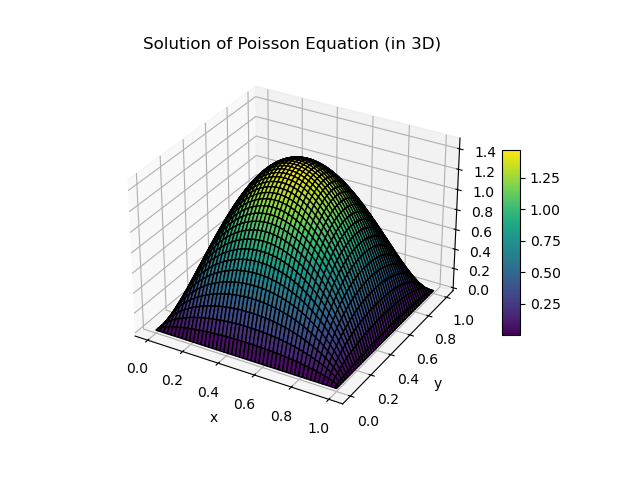
\includegraphics[width=\textwidth]{../src-5/poisson/solution_petsc_plot_3d.png} % Replace with your file
    \end{subfigure}
    \hfill % Adds horizontal space
    % Second image
    \begin{subfigure}[b]{0.45\textwidth} % Adjust width as needed
        \centering
        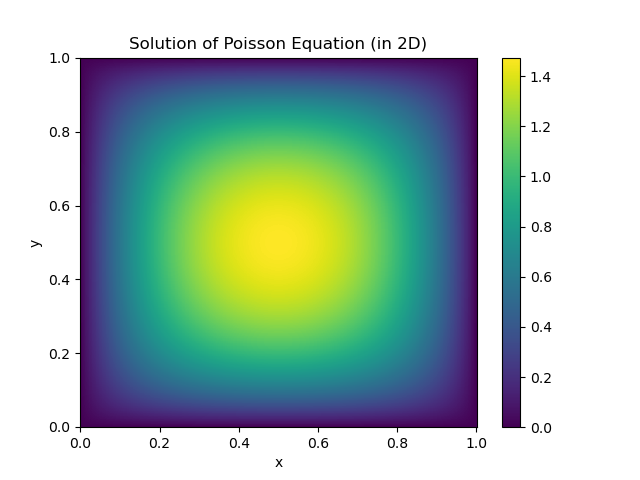
\includegraphics[width=\textwidth]{../src-5/poisson/solution_petsc_plot.png} % Replace with your file
    \end{subfigure}
    \caption{Solution of the Poisson equation using PETSc}
  \end{figure}
\begin{figure}[H]
\centering
% First image
\begin{subfigure}[b]{0.45\textwidth} % Adjust width as needed
	\centering
	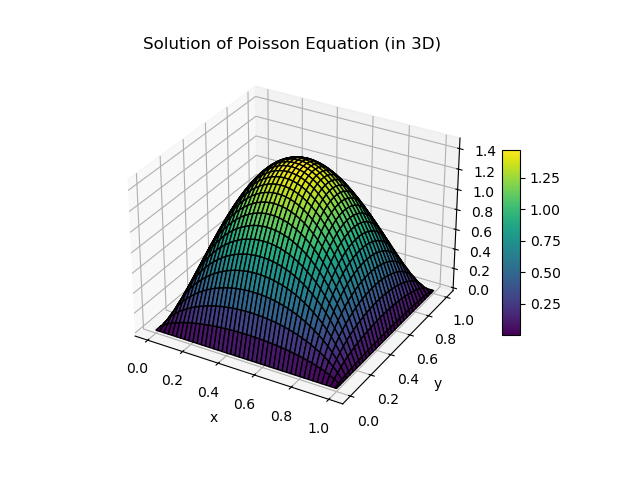
\includegraphics[width=\textwidth]{../src-5/poisson/solution_dn_dir_3d.png} % Replace with your file
\end{subfigure}
\hfill % Adds horizontal space
% Second image
\begin{subfigure}[b]{0.45\textwidth} % Adjust width as needed
	\centering
	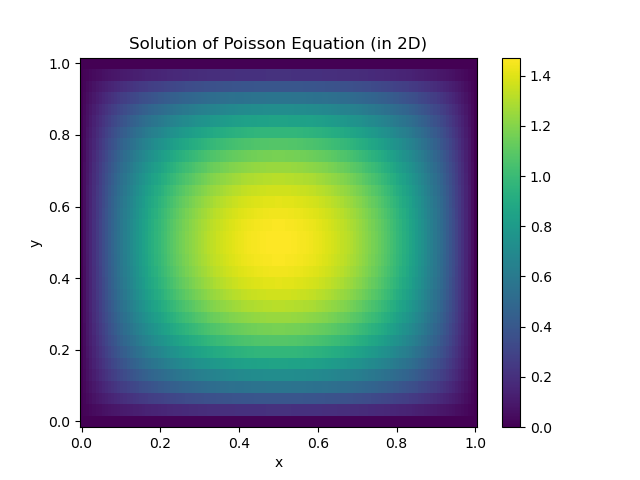
\includegraphics[width=\textwidth]{../src-5/poisson/solution_dn_dir.png} % Replace with your file
\end{subfigure}
\caption{Solution of the Poisson equation using Python Numpy dense solver solution plotted in 3D and 2D}
\end{figure}
\subsection{Performance Benchmark [15 points]}

\begin{figure}[H]
    \centering
    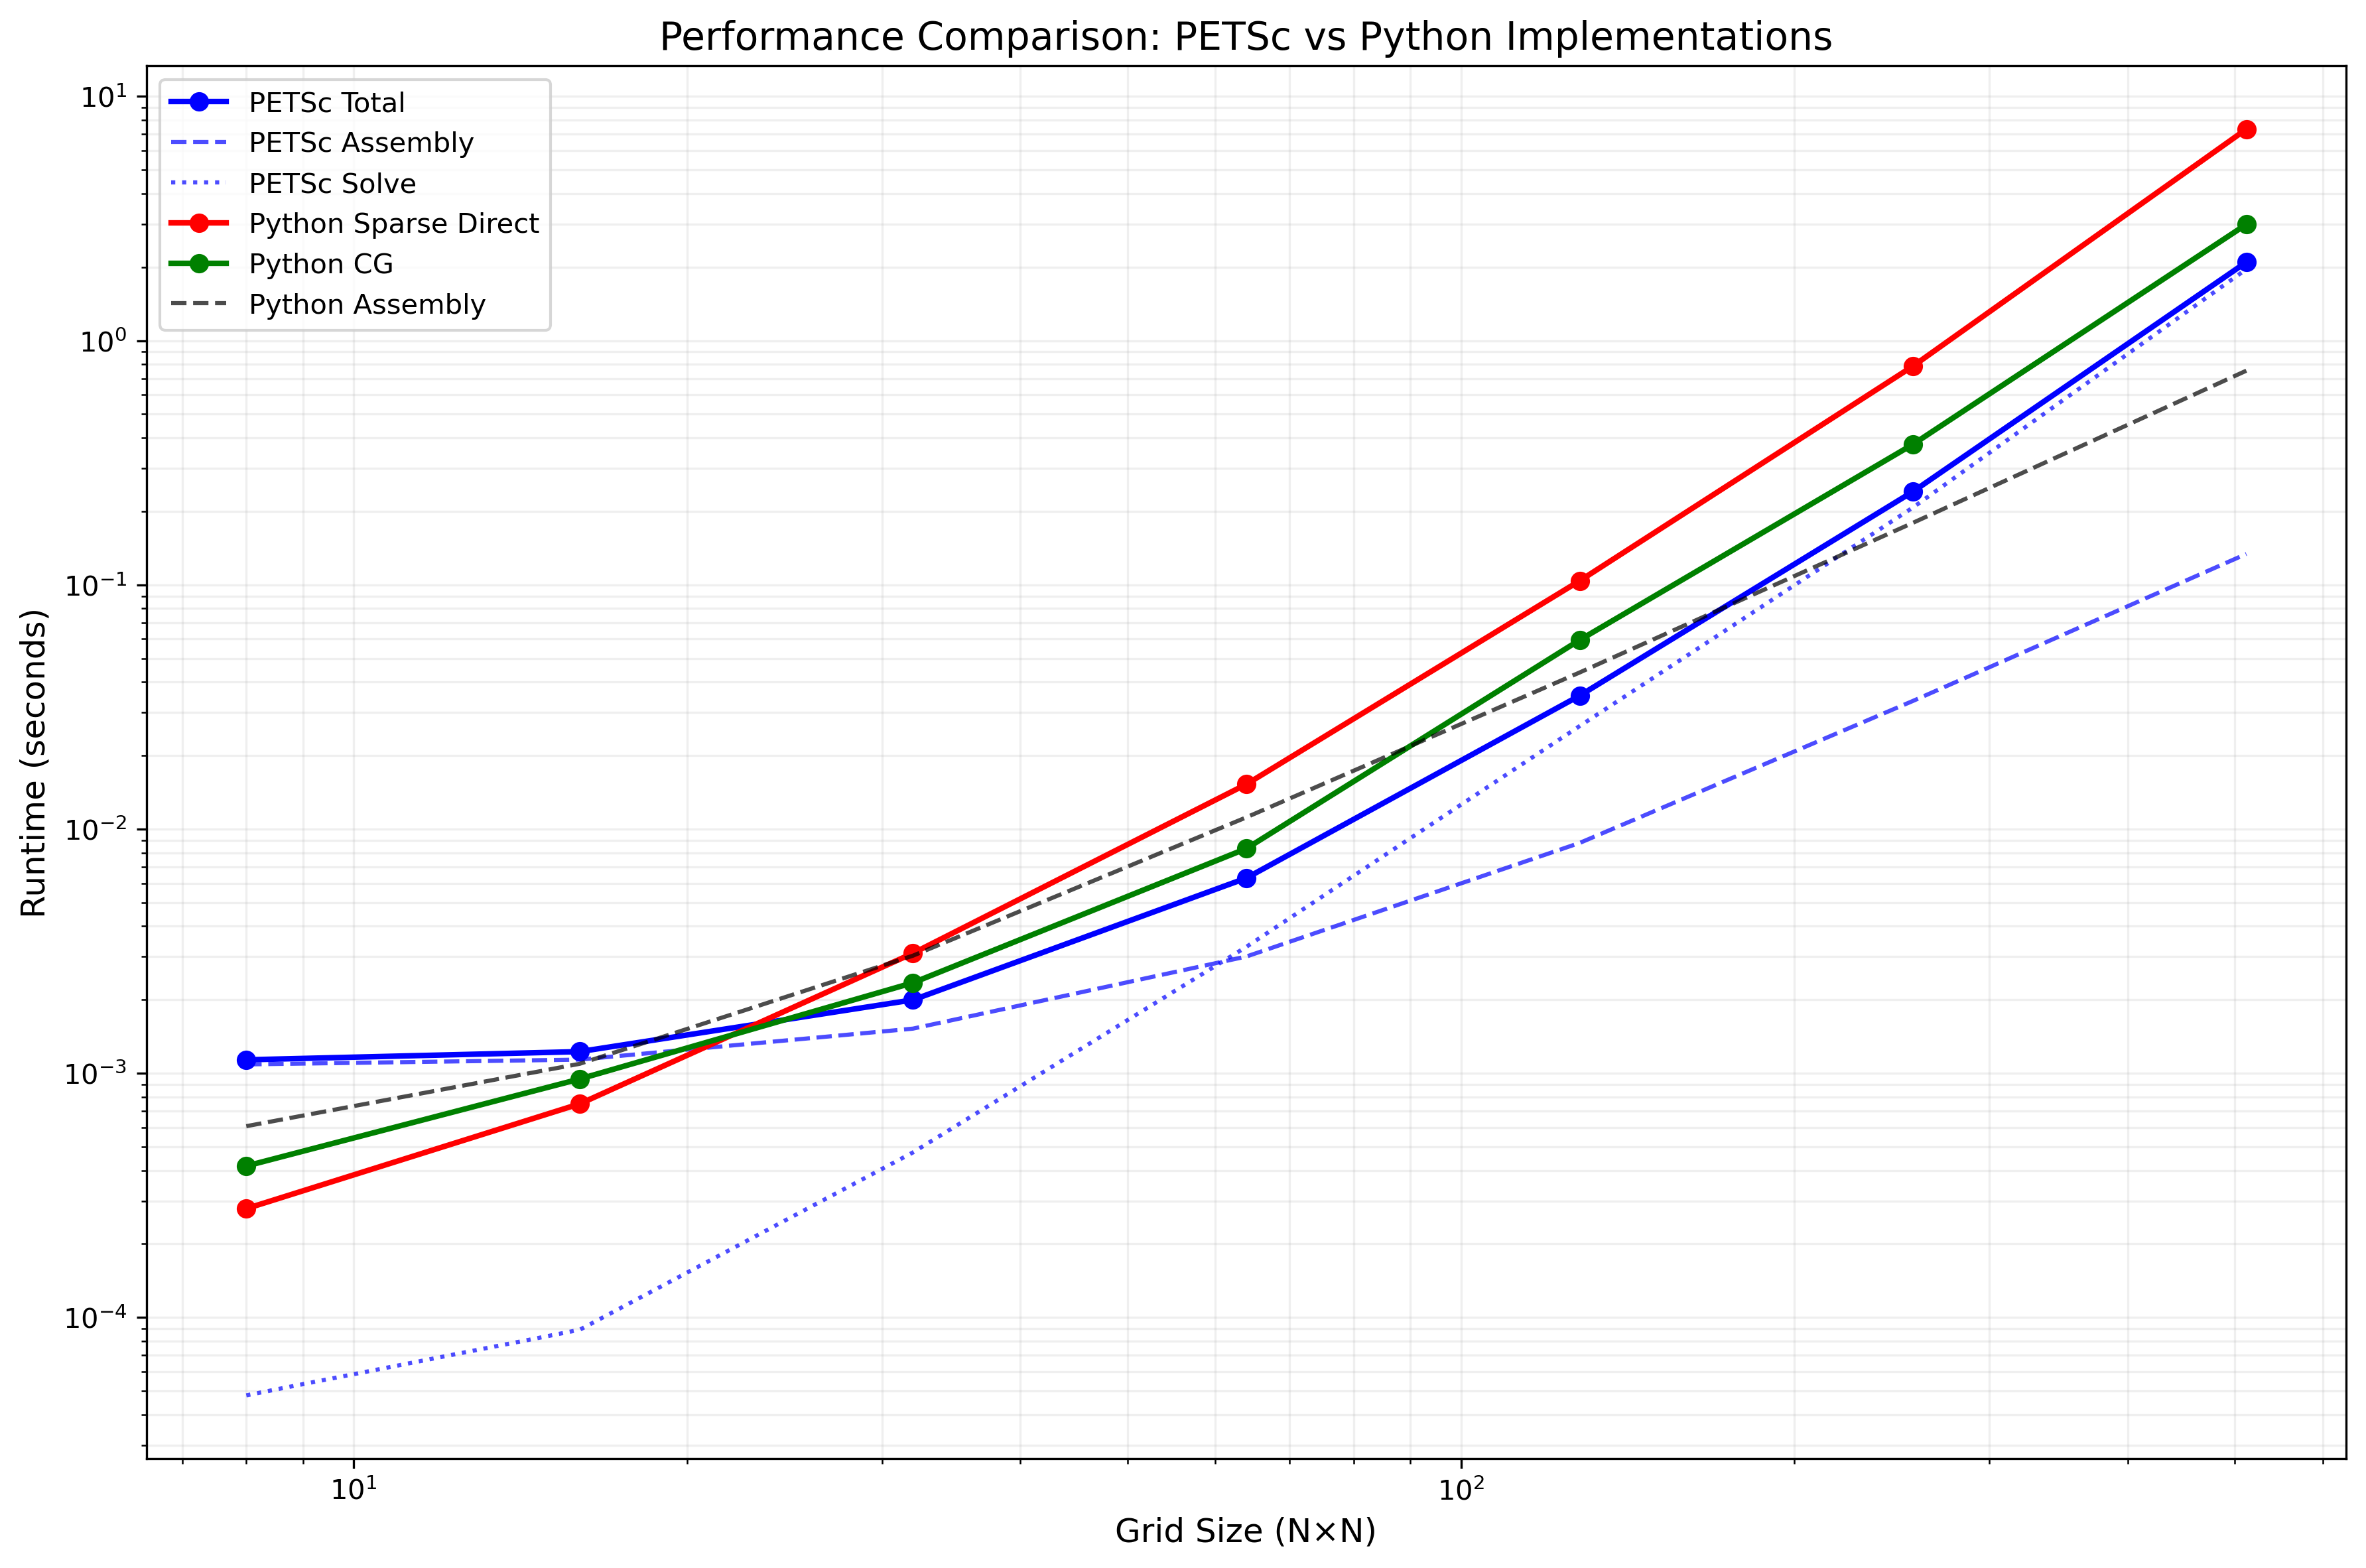
\includegraphics[width=\textwidth]{../src-5/poisson/test_perf/runtime_comparison.png} % Replace with your file
    \caption{Performance benchmark of the Poisson equation: Python vs PETSc}
\end{figure}
                     
The performance comparison between both implementations across different grid sizes (8x8 to 512x512) shows that 
PETSc consistently outperforms the Python implementation. 
For smaller grids, both implementations show similar performance, but as the grid size increases, 
PETSc advantage becomes more pronounced. 

\subsection{Strong Scaling [10 points]}

\begin{figure}[H]
    \centering
    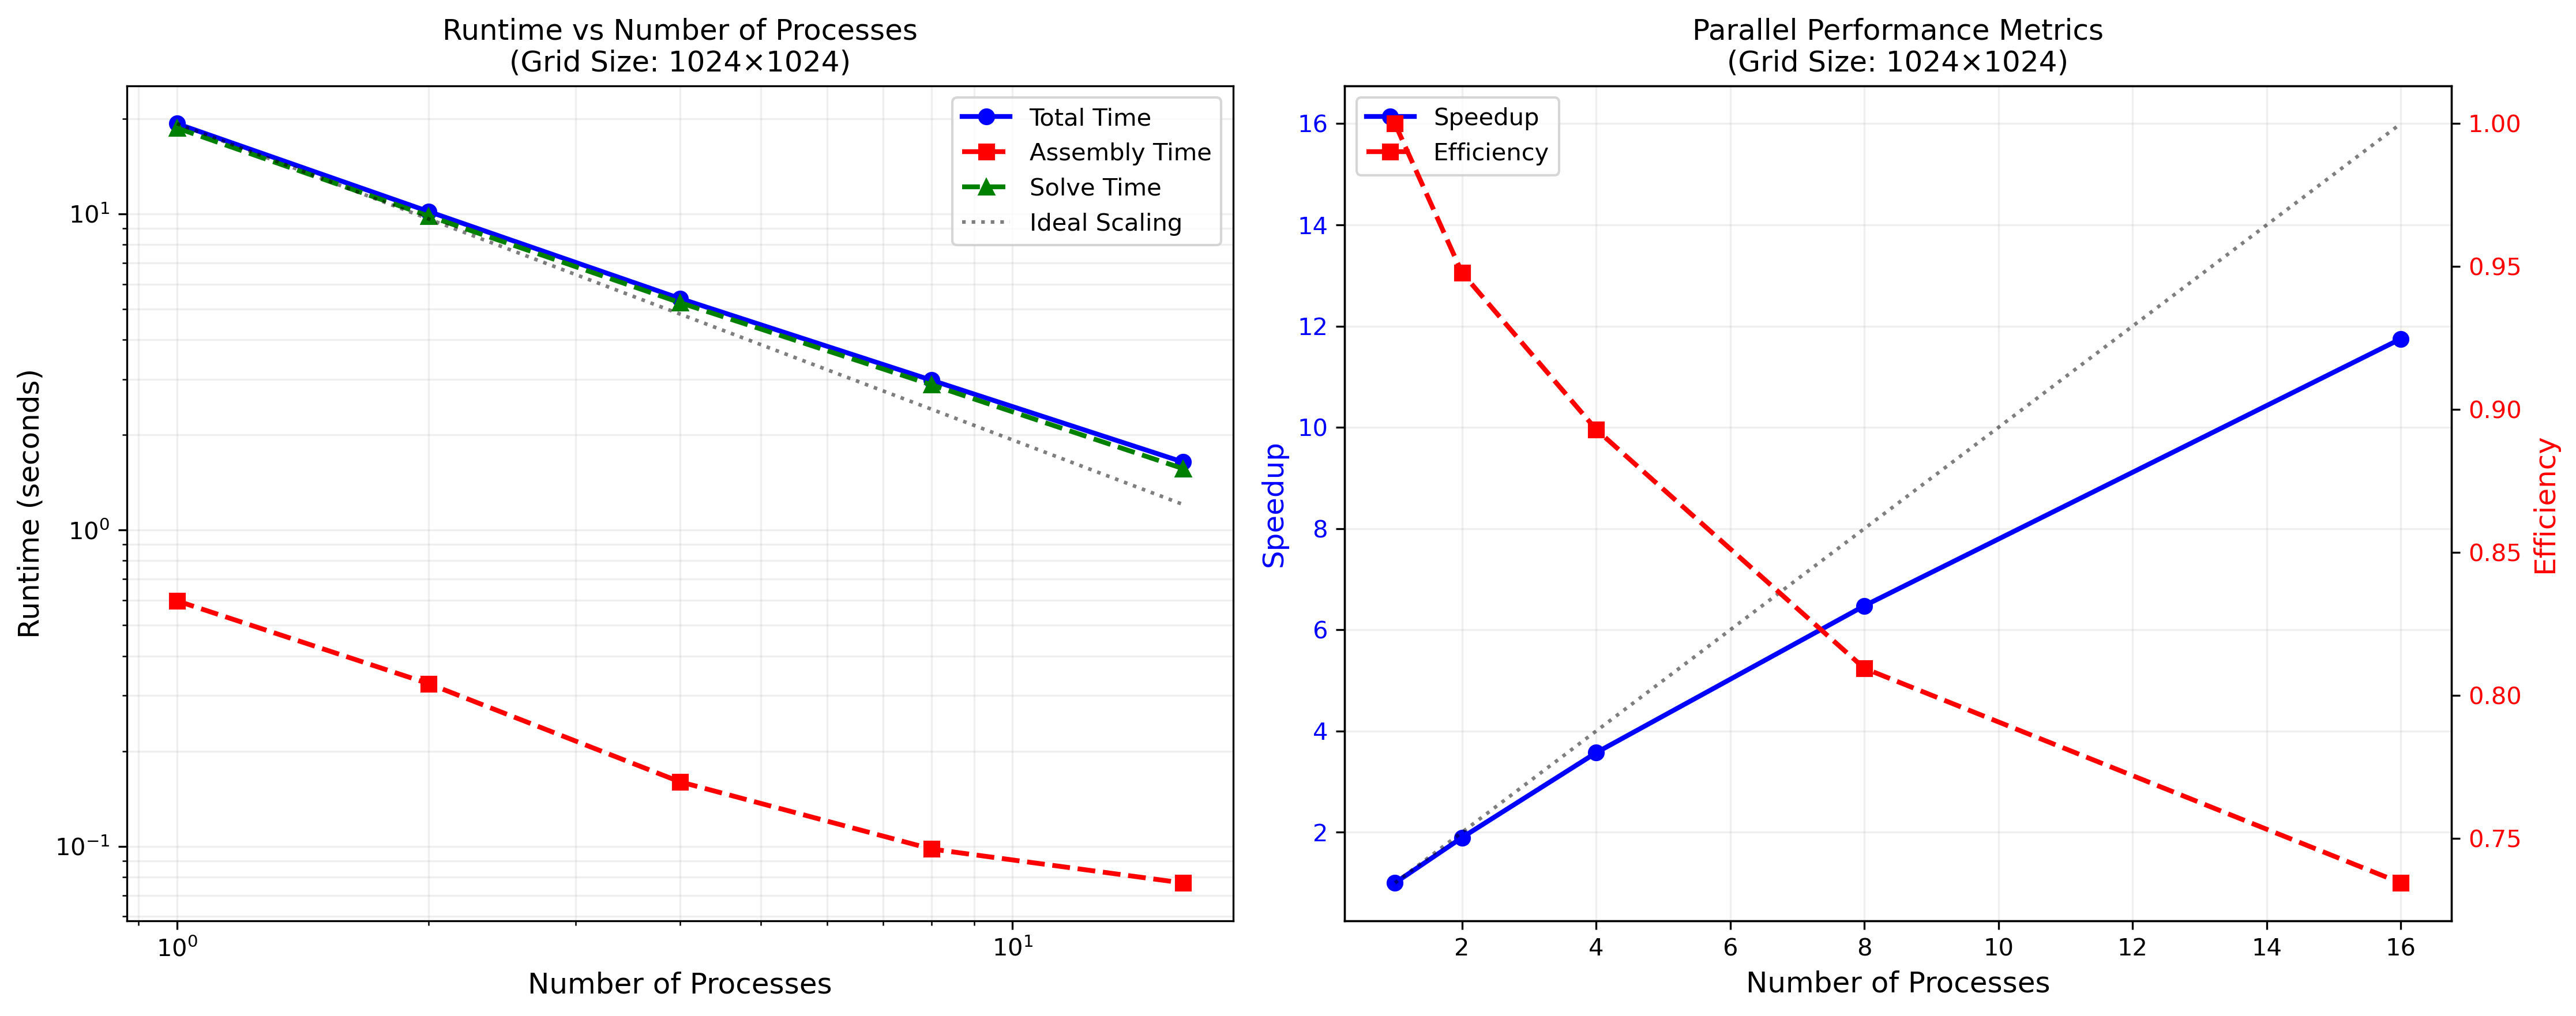
\includegraphics[width=\textwidth]{../src-5/poisson/test_scale/parallel_scaling.png} % Replace with your file
    \caption{Strong scaling of the Poisson equation: Python vs PETSc}
\end{figure}
The strong scaling test \footnote{fixed problem size 1024×1024 with increasing process count from 1 to 16} demonstrates good parallel efficiency for the PETSc implementation.
 The total runtime decreases from 19.29s (1 process) to 1.64s (16 processes), showing an approximate speedup of 11.76x. While not achieving perfect linear speedup (16×), 
 this is reasonable due to communication overhead. The assembly phase shows better scaling efficiency than the solve phase.

\end{document}
